\section{Evolution Management}
\label{sec:evolution-management}

Everything is subject to change, and multi-model data is no exception. Changes can occur in any part of the system, such as the conceptual schema, logical models, the data itself, or the queries. \term{Evolution management} involves detecting these changes, describing them in a formal way, and propagating them to all the affected components, so that we can maintain consistency and correctness of the system. The last part, \term{change propagation}, is especially challenging in a multi-model environment, where the relationships between components can be complex and the changes can have far-reaching consequences. Based on the related work (\Cref{sec:evolution-related-work}), we identified the following open questions:

\question{ep:smos}{Unified evolution}{There is a categorical approach to modeling multi-model data, offering a unified repesentation of all popular data models and their combinations. However, real-life datasets are rarely ever static. We should be able to evolve one model to another in an efficient way (i.e., without having to redefine the whole model from scratch). In order to do that, the change should be expressed as a set of atomic operations with clear preconditions and postconditions. Crucially, the evolution should work for all models in a uniform way despite their different features and semantics.}

\question{ep:smo-intent}{High-level operations}{Users usually interact with the system at a higher level of abstraction than atomic operations. For example, while moving a property from one entity to another can be decomposed to a sequence of basic operations, it is often beneficial to express it as a single high-level operation. This better captures the user's intent, allows for better optimization (a complex operation can usually be decomposed in several ways, some of which are more efficient than others), and also offers better error handling (if one atomic operations fails, we can roll back the whole complex operation, instead of having to deal with a partially applied change).}

\question{ep:data-propagation}{Propagation to data}{Once the schema of data is changed, the data must be changed as well to maintain consistency. A most straightforward approach would be to load all data to some universal representation, apply the change, and then transform it back to the original model. However, this is not efficient, especially for large datasets. Instead, we should be able to modify the data directly in the database via a sequence of \acrshort{ddl}/\acrshort{dml} statements. Ideally, we would find the most efficient sequence of statements for the given change.}

\question{ep:evolution-inference}{Change detection}{High variance and dynamicity is a common characteristic of modern data. We should be able to detect changes in the data and keep the models up-to-date. Additionally, multi-model data naturally supports redundancy, both intra-model (i.e., some NoSQL databases promote denormalization) and inter-model (i.e., same data can be represented in multiple models). Modifications to the data in one model (or part of it) should be reflected in the other models (or parts of them) to maintain consistency.}

\question{ep:query-propagation}{Propagation to queries}{A dataset consists not only of data, but also of queries defined over the data. When the schema changes, the queries must be adapted to ensure they still return the intended results. This is particularly challenging in a multi-model environment where queries may span multiple data models and their relationships can be complex.}

\question{ep:evolution-automation}{Evolution automation}{Some changes can be propagated automatically, while others require additional information (e.g., specific domain knowledge) to correctly interpret the user's intent. However, they should still be automated as much as possible. The user must be able to intervene the process at any point, but the system should be able to decide where to explicitly ask for user input, and where to automatically choose the best option.}

\question{ep:migration-strategy}{Migration strategy}{There are multiple strategies for propagating changes to the data (e.g., \term{eager}, \term{lazy}~\citep{scherzinger2013managing}, and \term{hybrid}~\citep{scherzinger2016nosql}) and for reconstructing queries~\citep{DBLP:conf/er/CaruccioPT18,DBLP:conf/foiks/Ravve16,DBLP:journals/corr/abs-2403-09060}. The best strategy depends on the specific situation, such as the size of the data, the frequency of queries, the expected performance impact, etc. The system should support multiple strategies to accomodate a wide range of use cases, and it should also be able to choose the most appropriate strategy based on the current workload and data characteristics.}

\subsection{Evolution Hierarchy}

A change in one component that is propagated to another component is also a change, so it may require further propagation, leading to a cascade of changes that can be difficult to manage. This is especially true in a multi-model data world, where there are many different components and relationships between them.

Our approach starts by defining a clear hierarchy of components and a set of rules for how changes should be propagated between them. On the top of the hierarchy (see \Cref{fig:evolution-hierarchy}), there is the conceptual schema. The schema can be edited via atomic operations, called \acrshort{smo}s, coming either directly from the user, or being automatically inferred from changes in the data (as mentioned in \Cref{sec:vision-automation}).

Next, the logical models can also be edited via \acrshort{smo}s (different ones than those used for the conceptual schema), which are automatically generated by propagating changes from the conceptual schema. The operations can be created directly as well---either by the same use cases as the conceptual changes (i.e., user-specified or data-driven), or by the last use case from \Cref{sec:vision-automation} (i.e., self-adaptation).

Changes in the logical models are propagated to the data via \acrshort{ddl} and \acrshort{dml} statements. However, these changes do not affect queries, as they are defined over the conceptual schema and only translated to the native database queries at execution time. So, the queries are updated directly by the conceptual \acrshort{smo}s.\\

This downwards approach (i.e., from the most abstract components to the most concrete ones) is not the only way to propagate changes. An upwards approach is also possible---either originating from the data or from the queries.

The former is done by observing changes in the data (e.g., a new field is added to a document collection) and inferring the corresponding \acrshort{smo}s that would have caused those changes. These \acrshort{smo}s are then applied to the conceptual schema and logical models, leading to the above-described downwards propagation to the data and queries.

The latter concerns only changes in the query \emph{workload}, not in the \acrshort{mmql} query contents---the queries depend on the conceptual schema, not the other way around. The system can observe shifts in the workload (i.e., the frequency of certain queries) and use that information to trigger self-adaptation, leading to further changes in the logical models and data.

\begin{figure}[ht]
    \centering
    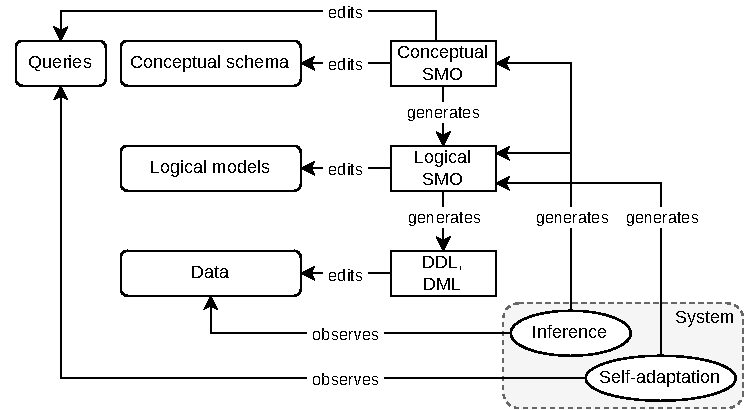
\includegraphics[width=\textwidth]{img/commentary-evolution_hierarchy.drawio.pdf}
    \caption{Hierarchy of components for evolution management. All changes are mediated by atomic operations (\acrshort{smo}, \acrshort{ddl}, \acrshort{dml}) which are propagated downwards. Direct changes originating outside of the system (i.e., data, query workloads) are observed and propagated upwards by inferring the corresponding atomic operations.}
    \label{fig:evolution-hierarchy}
\end{figure}

\subsection{Change Propagation}

The \acrshort{smo}s are formally defined in \paperRef{rcis_2025}. For clarity, we divide them into three groups based on the level of abstraction. The \term{basic} operations are atomic and work with individual objects and morphisms, e.g., \code{create}, \code{delete}, and \code{move}. The \term{composite} operations work with frequent higher-level patterns, such as properties, relationships, arrays, sets, or maps, e.g., \code{createProperty}, or \code{deleteMap}. Finally, the \term{complex} operations capture larger restructurings of existing schema fragments where several intermediate choices must be coordinated, e.g., \code{group}, \code{join}, or \code{asMap}. This division is important for propagation---users can work with expressive high-level commands, but the system can still reduce them to a sequence of basic operations with explicit preconditions and postconditions.

Once the change is expressed in this form, the system propagates it along the hierarchy described above. In \paperRef{rcis_2025}, we further distinguish between \term{light} and \term{heavy} propagation. A light operation only updates the mappings, whereas a heavy operation continues all the way to the logical schemas and data instances. This distinction is useful because not every conceptual change must immediately trigger a full data migration---some operations can remain only as logical adjustments until a heavier form of propagation is required.

Toward the queries, we build on the approach from \paperRef{edbt_2024}, where schema changes are reflected in \acrshort{mmql}. More specifically, each query is analyzed through its selection and projection categories, which capture the graph patterns and returned structure over the conceptual schema. The propagation then evaluates how a given basic \acrshort{smo} affects these categories and related clauses such as \code{FILTER}, \code{DISTINCT}, \code{ORDER BY}, or aggregations. As a result, some changes have no observable effect, some lead to a restricted rewrite with potentially changed semantics or performance, and some are too destructive to be repaired automatically. In the last case, the system must either ask for additional guidance or switch to a different propagation strategy.

\begin{example}
\label{ex:evolution-add}
Starting with the conceptual schema and columnar logical model (\Cref{fig:mapping}), the users might realize they want to be able to delete reviews. To do that, they use the \code{createProperty} operation to add a property \object{deletedAt} to the entity \object{Review} in the conceptual schema and connecte them via a new morphism (\signature{18}). This triggers the creation of the corresponding attribute in the logical model via the \code{updateMapping} operation, and the addition of the attribute to the data via the corresponding \acrshort{ddl} statements (\Cref{fig:evolution-add}).

Although the entity is used in the \acrshort{mmql} query from \Cref{fig:query-multi}, the change is not propagated there because adding a property does not affect the query results. However, the users might decide to add the property to the query manually, because they want to be able to filter out deleted reviews (\Cref{fig:query-propagation-multi}).
\end{example}

\begin{figure}[ht]
    \centering
    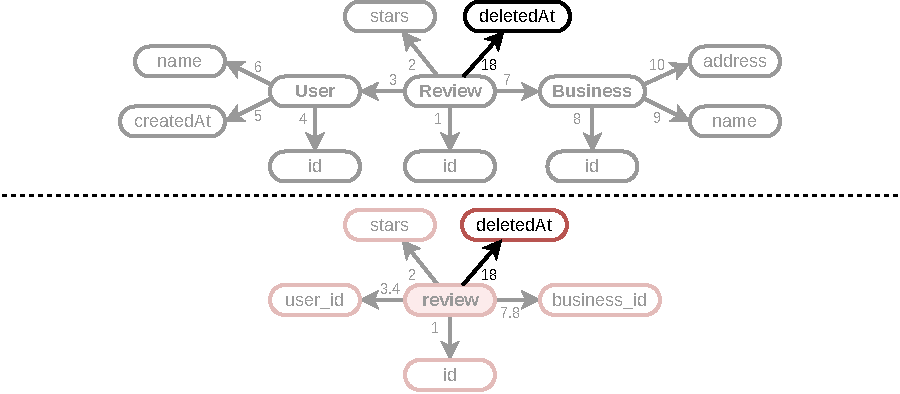
\includegraphics[width=\textwidth]{img/commentary-evolution_add.drawio.pdf}
    \caption{Schema from \Cref{fig:schema-category} is extended via the \code{createProperty} operation. The change is propagated to the logical model.}
    \label{fig:evolution-add}
\end{figure}

\begin{figure}[ht]
    \centering
    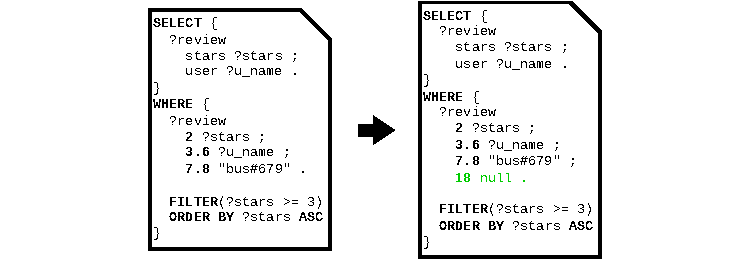
\includegraphics[width=\textwidth]{img/commentary-query_propagation_multi.drawio.pdf}
    \caption{The \acrshort{mmql} query from \Cref{fig:query-multi} is manually updated to include the new \object{deletedAt} property added in \Cref{fig:evolution-add}.}
    \label{fig:query-propagation-multi}
\end{figure}

\begin{example}
\label{ex:evolution-map}
A more complex use case is displayed in \Cref{fig:evolution-map}. Properties of the \object{Attributes} entity represent various characteristics of the businesses. In such a dynamic environment, it is common that new attributes are added to the data. In order to do that quickly, the users might decide to transform the entity into a key-value map via the \code{asMap} operation. The \object{Attribute}, \object{key}, and \object{value} objects are created, together with the morphisms \signature{19}, \signature{20}, and \signature{21}. Note that the morphism \signature{19} has the opposite direction than the previous morphism \signature{11}. This is because in the original schema, there was a \code{*:1} relationship between the \object{Business} and \object{Attributes} entities. Now, there is an \code{1:N} relationship between the \object{Business} and \object{Attribute} entities (one business can have multiple attributes).

After that, the old \object{Attributes} entity is deleted. The logical model is updated accordingly. This time, the change does affect the query from \Cref{fig:query-single}, because the \object{Attributes} entity was used in the query. The query is rewritten to use the new objects instead, and the previous attributes are replaced with explicit string literals, filtering the \object{key} properties (\Cref{fig:query-propagation-single}).
\end{example}

\begin{figure}[ht]
    \centering
    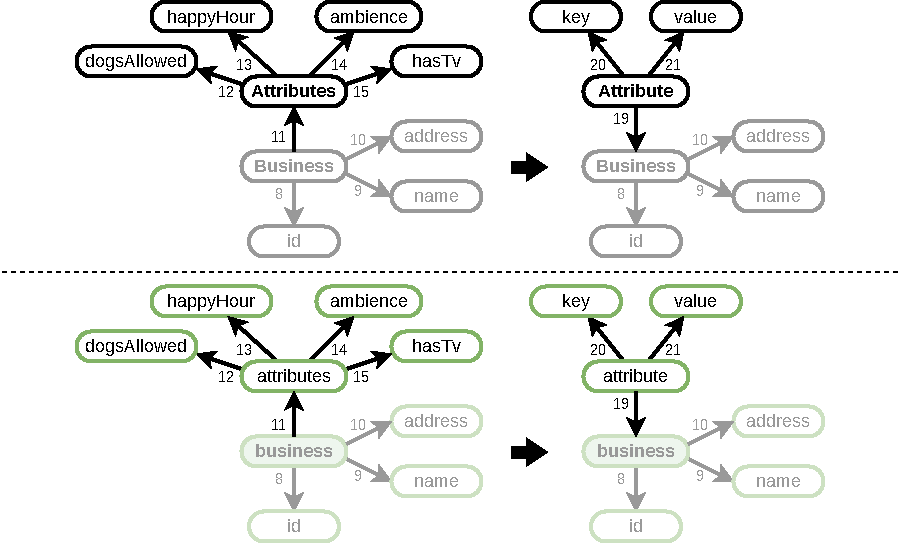
\includegraphics[width=\textwidth]{img/commentary-evolution_map.drawio.pdf}
    \caption{Schema from \Cref{fig:schema-category} is transformed via the \code{asMap} operation. The change is propagated to the logical model.}
    \label{fig:evolution-map}
\end{figure}

\begin{figure}[ht]
    \centering
    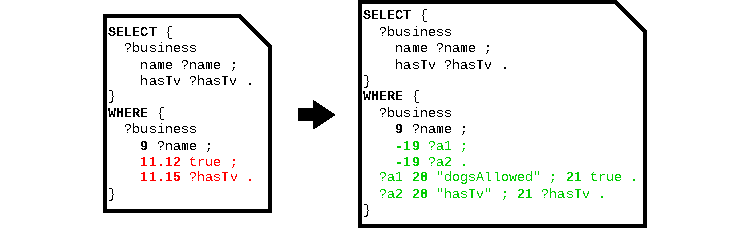
\includegraphics[width=\textwidth]{img/commentary-query_propagation_single.drawio.pdf}
    \caption{The \acrshort{mmql} query from \Cref{fig:query-single} is automatically fixed so that it uses the new \object{Attribute} map created in \Cref{fig:evolution-map}.}
    \label{fig:query-propagation-single}
\end{figure}

Because the propagation is defined over atomic operations, we do not have to execute the whole change in a single step. Composite and complex operations can be decomposed, analyzed, and then propagated incrementally, which makes it possible to interleave the process with additional user input whenever some intermediate choice requires domain knowledge. The same decomposition is useful for scheduling---individual propagation steps can be postponed to a more suitable moment, e.g., when the system is underutilized, without losing track of the overall intent of the change. Regarding the data itself, our current implementation assumes eager migration, i.e., all affected records are updated immediately. Nevertheless, the framework is not tied to this choice. In principle, it can also support lazy or hybrid strategies by maintaining access to older versions of the conceptual schema, logical models, and queries until the migration is completed.

\subsection{Level of Automation}
\label{sec:evolution-automation}

As mentioned in \Cref{sec:vision-automation}, the process of change propagation can be automated to different degrees.
\todo{toto nezní vědecky

The more automation, the less manual work and expertise is required from users, but also the less control they have over the process.}

\todo{Co to je??? Teoreticky budemeněkd lítat na Venuši. }
In theory, the entire process could be fully automated with a sufficiently advanced AI system that can understand the semantics of the data and queries, predict the impact of changes, and make the best decisions about how to propagate them. In practice, we are still far from achieving this level of automation, and there are many challenges to overcome before we can get there. Therefore, we automate the process gradually following three distinct levels~\citep{ideas2022vision}.

\subsubsection{Rule-based Adaptation}

\todo{Tato kapitola ale nikde nevysvětluje, co to je teda rule-based adaptace.}

In the first level, we define the \acrshort{smo}s and their propagation rules. This is the case of \Cref{ex:evolution-add,ex:evolution-map}. Another use case would be to use the \code{createMapping} operation to define a new mapping between the conceptual schema and a logical model, e.g., a graph model, triggering the transformation of the data to the new model.

The above-described operations are deterministic and have strict preconditions and postconditions, so we can be sure that they will always lead to a consistent state of the system. However, this means there is a lot of situations that cannot be handled by the system. E.g., if a property is deleted and a certain query depends on it, there are several ways to rewrite the query, but none of them is strictly correct or incorrect. In such cases, a manual intervention is required to choose the preferred option. This approach is explained in detail in \paperRef{edbt_2024}. \todo{Ale tady by mělo být nějak vidět, co jsem v tom paperu vyřešili.}

\subsubsection{Learning-based Adaptation}

This level builds on top of the previous one by leveraging the deterministic operations and rules, but also using AI techniques to decide \emph{which} operations to apply in situations where there are multiple options. These techniques range from simple heuristics to more complex machine learning models that can learn from past examples and make informed decisions about how to propagate changes.

\todo{víc detailů}
For example, \paperRef{rcis_2025} discusses several query propagation strategies that can be applied when a property is deleted, and evaluates their performance on a real-world dataset. The system can learn from the observed workload and data characteristics to choose the most appropriate strategy for each situation.

Tasks like this rely heavily on detailed insights about the workload and data. \todo{Toto je velký skok, to nikdo nepochopí. In the case of query propagation, functional dependencies between attributes are particularly useful, as they can help to identify which attributes are likely to be affected by a change and how to rewrite the queries accordingly.} This is the main motivation behind our new approach designed to not only discover functional dependencies, but to also distinguish between genuine, fake, and ghost dependencies. The approach, together with a proof-of-concept implementation called \term{FDepHunter}, is described in \paperRef{vldb_2025_fdephunter}.

Rather than treating dependency discovery as a fully automatic black-box task, FDepHunter provides an interactive workflow in which domain experts iteratively refine the discovered dependencies. Technically, it incrementally builds an Armstrong relation~\citep{DBLP:books/aw/AbiteboulHV95} enriched with positive and negative examples, which approximate the relevant properties of the complete dataset while allowing several questionable dependencies to be refined at once. This gives the system a practical way to obtain higher-quality semantic information in situations where purely automatic profiling would be too unreliable for downstream adaptation tasks.

\subsubsection{Self-adaptation}
\todo{Nechápu, proč je to tady a pak znova dál.}

Instead of reacting to changes by \uv{repairing} parts of the system whenever other parts change, a self-adaptating system proactively tries to optimize its overall performance. This involve finding the right balance between the cost of and performance benefits of transforming the data to a different model, and rewriting the queries to take advantage of the new model. This is a very complex task that requires deep understanding of the workload and data characteristics, as well as the ability to predict the impact of changes on the system's performance.

Another form of self-adaptation is to anticipate changes before they even happen. For example, a certain set of queries might not be frequently used now, but the changes of this frequency might suggest much higher usage in the future, so the system can adapt itself in advance. These concepts are further explored in \Cref{sec:self-adaptation}.

\subsection{Related Work}
\label{sec:evolution-related-work}

\todo{RELATED WORK}


\subsection{Contributions}

We proposed a novel approach to evolution management in multi-model data management systems. It is based on a unified categorical representation of multi-model data, which allows us to include all popular data models and their combinations in a single framework. Thanks to the shared abstraction over logical models, we can express analogous modifications uniformly instead of redefining them separately for each model, which improves both the expressiveness and the compactness of the overall operation set.

We defined a comprehensive set of atomic operations for modifying the conceptual schema, logical models, data, and queries (\questionRef{ep:smos}). These operations can be propagated between all components of the system in a systematic way (ensuring consistency and correctness) and with different levels of automation (reducing manual work and expertise required from users) (\questionRef{ep:evolution-automation}).

Besides the atomic operations, we also defined more user-friendly composite and complex operations (\questionRef{ep:smo-intent}), which are reduced to the atomic ones during propagation. They can be used to express common changes in a more natural way, while still being propagated through the system in a consistent manner.

Another contribution is the extension of our evolution-management approach to query synchronization (\questionRef{ep:query-propagation}). When schema changes are propagated through the system, the corresponding queries must also be adapted so that they preserve their intended results whenever possible. We focused especially on situations with decreasing information capacity, where some information may be removed or become unavailable after the change. For these cases, we investigated several rewriting and synchronization strategies in the multi-model context and show how they fit into the broader evolution process.

Finally, we validated the proposed ideas through a proof-of-concept implementation and experimental evaluation. The implementation demonstrated that a substantial part of the evolution process can be handled systematically, reducing manual and error-prone intervention when propagating changes across schemas, mappings, data, and queries. The experiments then compared the efficiency of the considered synchronization strategies and provided initial evidence of the practical feasibility of the approach.\\

Another, more focused contribution is FDepHunter, which strengthens the learning-based part of our approach by providing better information about functional dependencies in real-world data. Although this is only a partial solution, it fits the broader evolution framework naturally---such dependencies provide exactly the kind of semantic insight needed for ambiguous query synchronization tasks and other situations where purely rule-based propagation is no longer sufficient. In this sense, FDepHunter is not a standalone side result, but a supporting component that improves the system's ability to make informed adaptation decisions.
